
  \begin{center}
    \begin{tikzpicture}[scale=0.5]
%      \tikzstyle{every node}=[color=white]
      \filldraw[fill=blue!50!black] (0,10) rectangle (5,8);
      \filldraw[fill=green!50!black] (13,10) rectangle (18,8);
      \filldraw[fill=blue!50!black,rounded corners=2mm] (0,5) rectangle (5,0);
      \filldraw[fill=green!50!black,rounded corners=2mm] (13,5) rectangle (18,0);
      \filldraw[fill=gray] (2,8) -- (2,5) -- (3,5) -- (3,8) -- cycle;
      \filldraw[fill=gray] (15,8) -- (15,5) -- (16,5) -- (16,8) -- cycle;
      \filldraw[fill=gray] (2,0) -- (2,-3) -- (16,-3) -- (16,0) -- (15,0) -- (15,-2) -- (3,-2) -- (3,0);
      \draw[color=white] (2.5,9) node {CPU Memory};
      \draw[color=white] (15.5,9) node {GPU Memory};
      \draw[color=white,font=\large] (2.5,2.5) node {CPU};
      \draw[color=white,font=\large] (15.5,2.5) node {GPU};
      \only<1>{
        \draw[font=\large] (9,-1.5) node {PCIe};
      }
      \only<2>{
        \draw[font=\footnotesize] (9,8) node {For every parallel operation};
        \draw[font=\footnotesize] (8,7) node {1: Move data from};
        \draw[font=\footnotesize] (8.5,6) node {Host to Device};
        \draw[font=\footnotesize] (7.7,5) node {2: Execute once};
        \draw[font=\footnotesize] (8.5,4) node {on the Device};
        \draw[font=\footnotesize] (8,3) node {3: Move data back};
        \draw[font=\footnotesize] (9.5,2) node {from Device to Host};
        \draw[font=\footnotesize] (9,0) node {What if we separate};
        \draw[font=\footnotesize] (9,-1) node { the data and Execution?};
      }
      \only<3>{
        \draw[font=\footnotesize] (6,8) node {Now};
        \draw[font=\footnotesize] (8,7) node {1: Move data from};
        \draw[font=\footnotesize] (8.5,6) node {Host to Device};
        \draw[font=\footnotesize] (9,5) node {only when needed}; 
        \draw[font=\footnotesize] (9,4) node {2: Execute multiple times};
        \draw[font=\footnotesize] (8.4,3) node {on the Device};
        \draw[font=\footnotesize] (8,2) node {3: Move data back};
        \draw[font=\footnotesize] (9.2,1) node {from Device to Host};
        \draw[font=\footnotesize] (8.3,0) node {when needed};
      }
    \end{tikzpicture}
  \end{center}
